\chapter{The ALICE Experiment}
ALICE (\textit{A Large Ion Collider Experiment}) is one of the four major experiments at the \textit{Large Ion Collider}, at CERN, in Geneva. It was expressly designed to study heavy ion collisions, continuing the tradition of experiments such as STAR and PHENIX at RHIC, but also experiments held at SPS and AGS before. The aim of the experiment is the study of the QGP, using Pb-Pb collisions. ALICE has also a program with data from p-p and p-Pb collisions, needed to discern final state effects from initial states effects.\\
In this chapter a description of the experimental set up will be given, focusing on the \textit{Inner Tracking System}, the detector on which this work is based, after a brief introduction about the LHC.
\section{Large Hadron Collider}
%
\begin{figure}
  \centering
  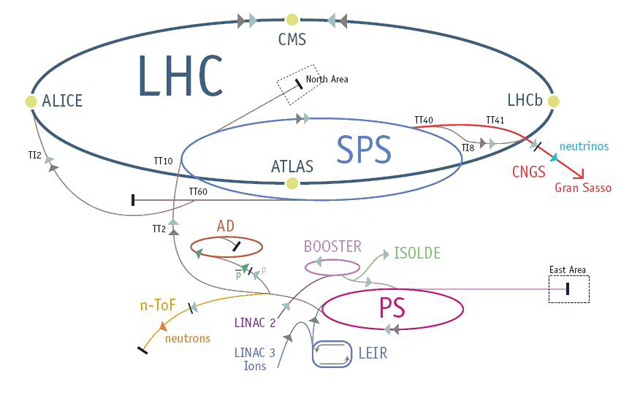
\includegraphics[scale=0.55]{figures/LHC.jpg}
  \caption{The accelerator complex at CERN.}
  \label{fig:LHC}
\end{figure}
%
The LHC is the world's largest and most powerful accelerator \cite{lhc}. It consists of a 27 km ring of superconducting magnets with a number of accelerating structures to boost the energy of the particles up to their collision energy and keep them stable, compensating the energy loss. The LHC is designed to deliver p-p collisions at $\sqrt{s}$ = 14 TeV, with a rate of 40 MHz, and Pb-Pb collisions at $\sqrt{s_{NN}}$ = 5.5 TeV, with a rate of 8 kHz. However, in the first run the LHC did not work at the highest energy, collecting mainly data for p-p collisions at $\sqrt{s}$ = 7 TeV and Pb-Pb collisions at $\sqrt{s_{NN}}$ = 2.76 TeV. In the second run, instead, the LHC is working at the design energies.\\
In Figure \ref{fig:LHC} a schematic view of the accelerator complex of CERN is shown. Protons and lead ions pass through different processes before reaching the LHC. Starting from protons, they are extracted from an hydrogen tank and injected in the linear accelerator LINAC2, where they reach an energy of 50 MeV. Then, they are accelerated to 1.4 GeV in the \textit{Proton Synchrotron Booster} (PSB) and injected in the \textit{Proton Synchrotron}, where they reach an energy of 25 GeV. Then, in the \textit{Super Proton Synchrotron} (SPS) they reach 450 GeV and are finally injected in the LHC. For lead ions the process is different, in particular in the initial steps. First of all, lead (Pb$^{208}$) ions are extracted from a purified sample of lead brought to high temperatures ($\sim$ 500 \textdegree C) thanks to microwaves and the partially ionized by a stream of electrons, creating ions with different charges, among which only Pb$^{29+}$ are selected. After being accelerated in LINAC3 at 4.2 MeV per nucleon, more electrons are stripped by passing through a carbon foil. Only Pb$^{54+}$ are kept end then accelerated in the \textit{Low Energy Ion Ring} (LEIR) at 5.9 MeV. Afterwards the ions are transferred to the PS, where they reach the energy of 5.9 GeV per nucleon end then pass through a copper foil, being fully stripped. The beam of Pb$^{82+}$ is then injected in the SPS (177 GeV per nucleon) and finally in the LHC, where they reach their final energy.
\section{Design considerations for ALICE}
The multiplicity of produced particles is a very important characteristic in the heavy ion collision experiments. For these kinds of studies, indeed, it is important to track and identify all the particles coming from the interaction region, in order to measure the quantities described in the previous chapter. As already mentioned, the ALICE experiment was designed when RHIC data were not available yet, and the estimated multiplicity for heavy ion collision at the energy of the LHC was 2000 - 6000 charged particles per rapidity unit. Consequently, the ALICE experiment has been designed in order to bear a multiplicity of 8000 particles per rapidity units. When the RHIC measurements became available, they showed that the multiplicity range at LHC should have been 1500 - 4000 particles for rapidity unit. Therefore, the designed was optimized for $\frac{dN}{dy}\sim$ 4000. The low interaction rate for heavy-ion collisions allows to use slow detectors, such as the time projection chamber and the silicon drift detectors, which are very suitable for the particle identification even at a high value of multiplicity.
Another important parameter that has been taken into account in the design of the experiment is the product of the efficiency, defined as the ratio between detected particles and generated particles, by the acceptance. ALICE is hermetic in $\varphi$, i.e. it covers $2\pi$ radians in the azimuthal angle.\\
ALICE, moreover, has been designed to work on a wide $\pt$ range. Thanks to the mild magnetic field (0.5 T), it is possible to track particles down to very low values of transverse momentum (tens of MeV). This feature is ideal for the study of particles with low momentum, but the combination of the chosen magnetic field with the long lever arm of the detector allows precise momentum measurements even at high momentum ($\pt\lesssim$ 100 GeV/c).\\
Beside the reconstruction of the trajectories of the charged particles, the particle identification (PID) is extremely important to reconstruct the particle spectra. At the ALICE experiment, the identification of particles with low transverse momentum ($\pt$ < 4 GeV/c) is performed in the central barrel ($|\eta|$ < 0.9). For higher momenta, the particle identification can be done just in a restricted range of $\eta$ and $\varphi$ by specialized detectors.
\section{ALICE experimental apparatus}
%
\begin{figure}
  \centering
  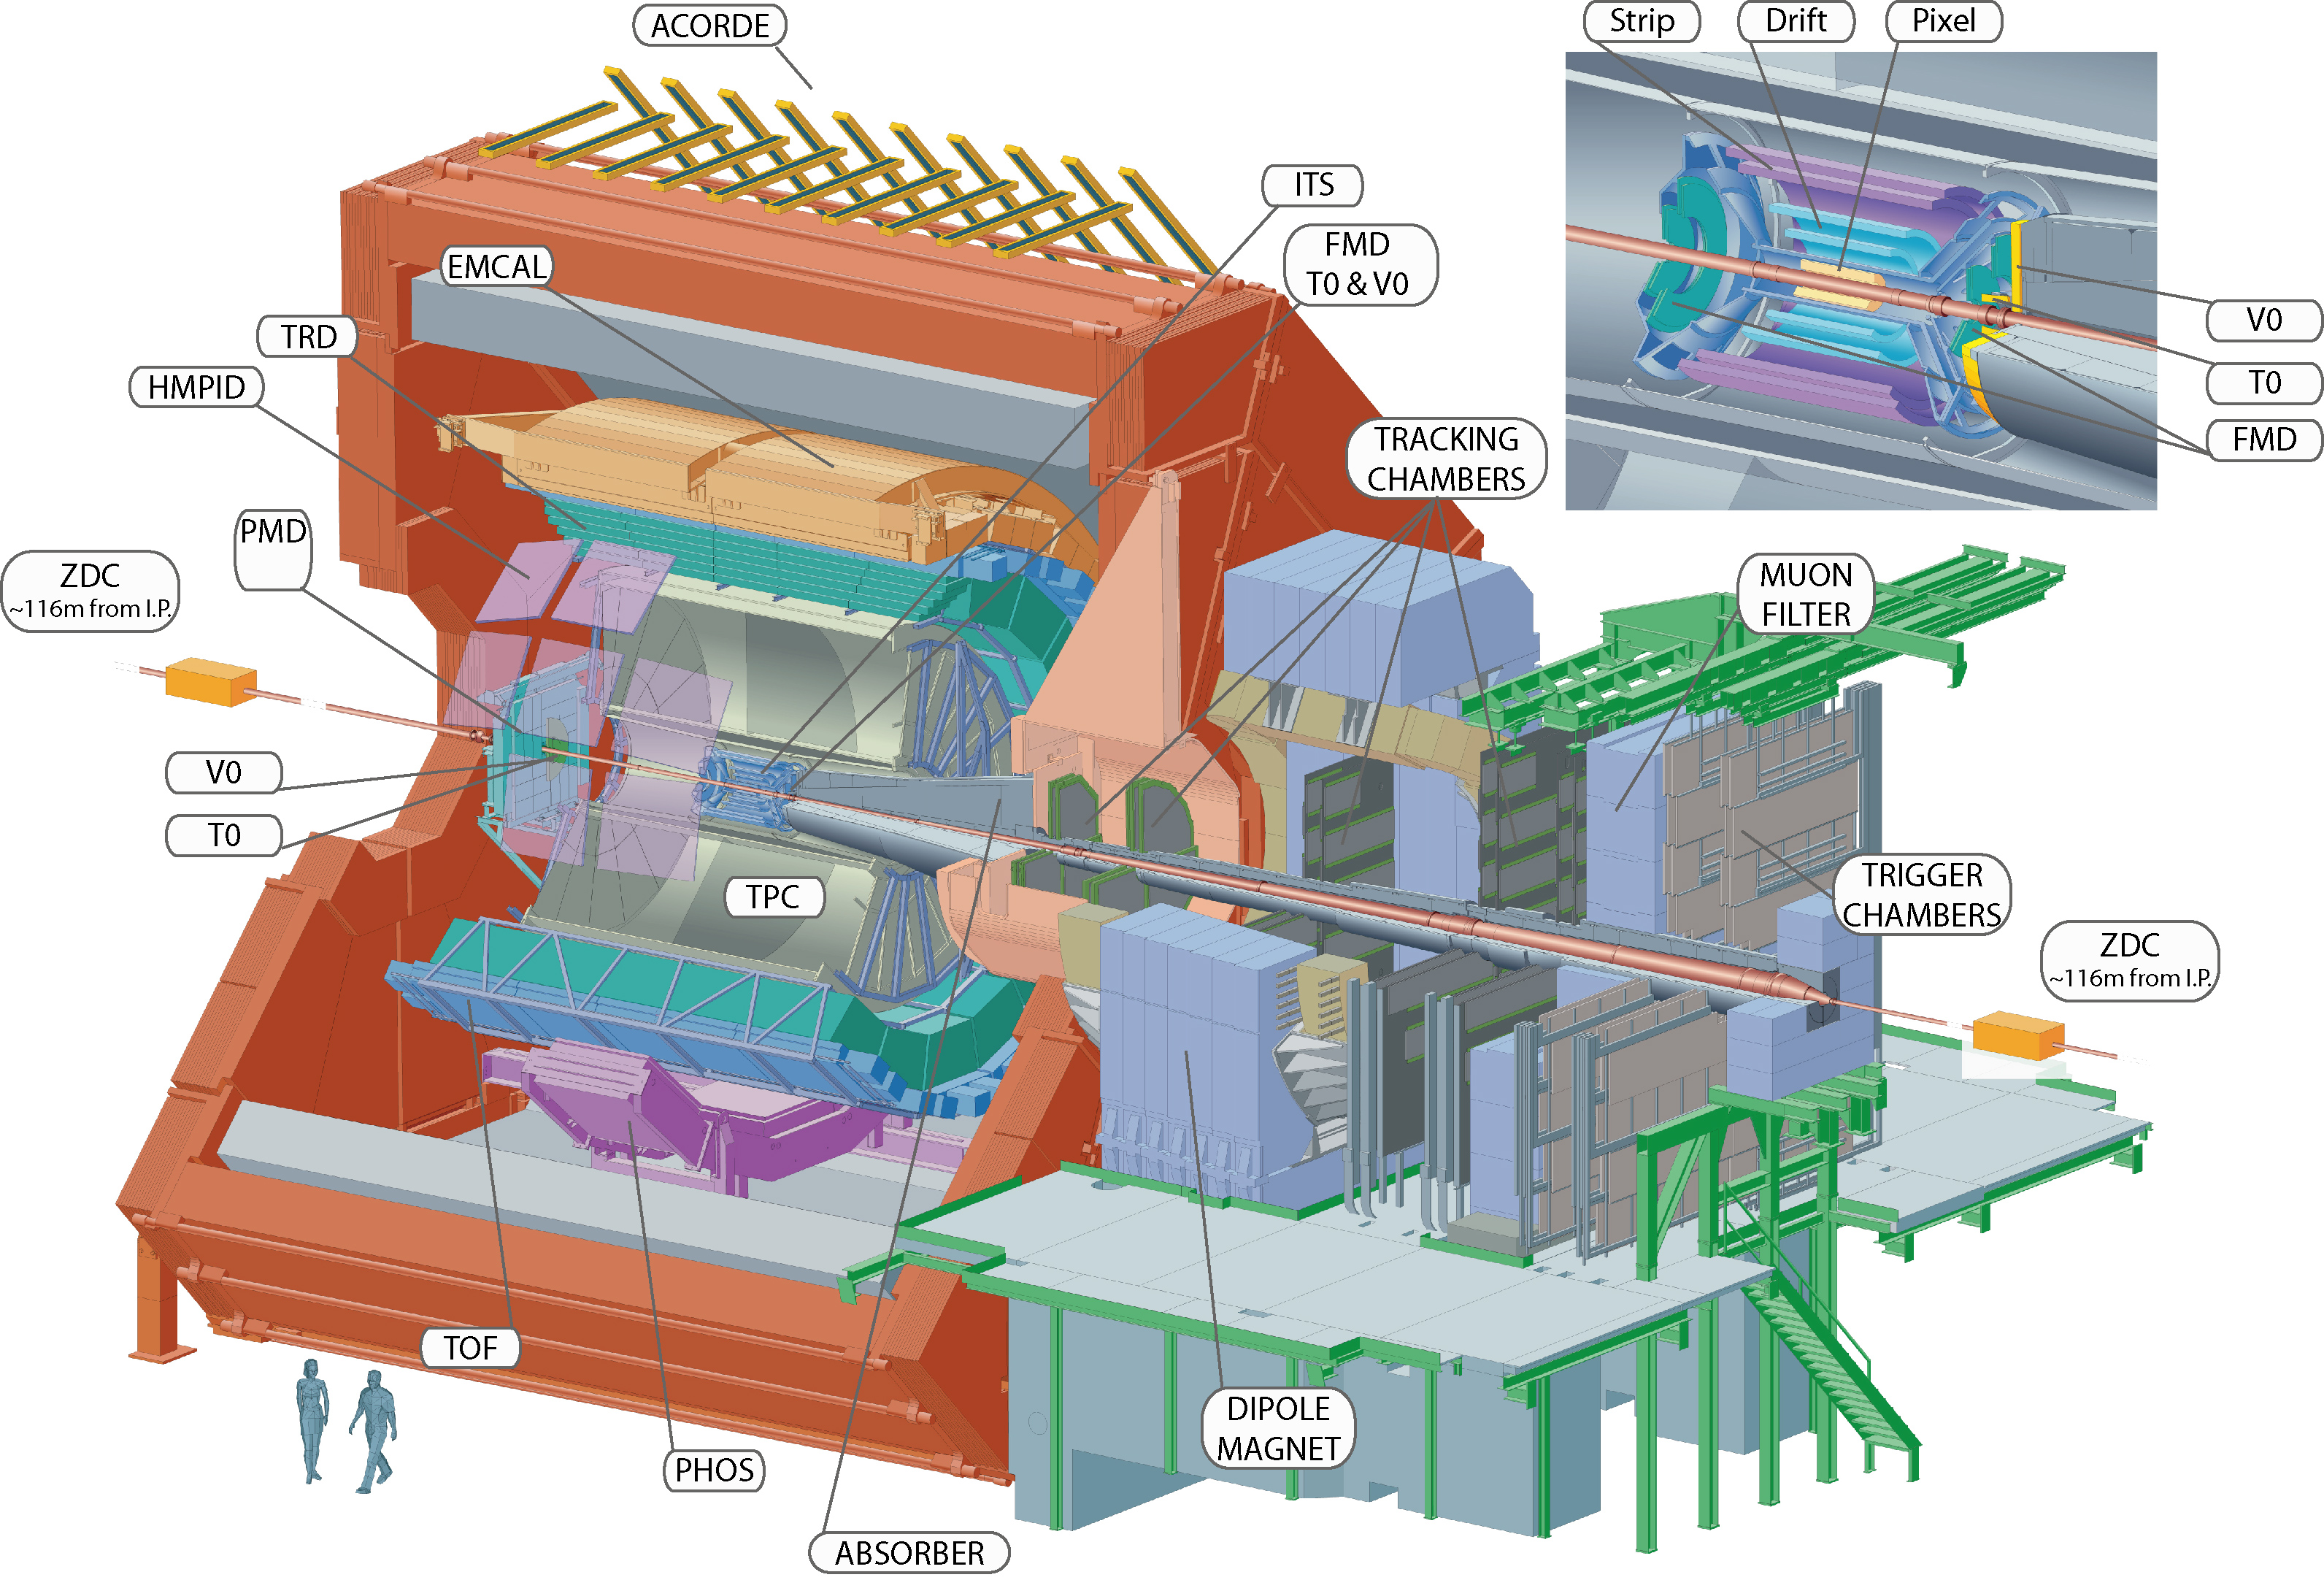
\includegraphics[scale=0.55]{figures/ALICEapp.jpg}
  \caption{The ALICE experimental setup.}
  \label{fig:ALICEapp}
\end{figure}
%
The experimental setup of ALICE is shown in figure \ref{fig:ALICEapp}. It is composed of three main parts: the \textit{central barrel}, which covers the mid-rapidity region (|$\eta$|<0.9), the \textit{muon arm}, which covers the forward pseudorapidity range -4 $\leq \eta \leq$ -2.5, and the \textit{forward detectors}.\\
All the detectors in the central barrel are immersed in the magnetic field of 0.5 T, generated by the ALICE solenoid magnet, used previously in the L3 experiment at the Large Electron-Positron (LEP) collider. The detectors of the central barrel, starting from the beam line and going outwards, are: the \textit{Inner Tracking System} (ITS), the \textit{Time Projection Chamber} (TPC), the \textit{Transition Radiation Detector} (TRD), the \textit{Time Of Flight} (TOF), the \textit{High Momentum Particle IDentification} detector (HMPID), the \textit{PHOton Spectrometer} (PHOS), the \textit{ElectroMagnetic Calorimeter} (EMCal) and the \textit{ALICE COsmic Ray DEtector} (ACORDE).\\
In the muon arm there is the \textit{Muon Spectrometer}, a forward detector which lays outside the solenoid magnetic field.\\
Finally the forward detectors, which are located at a small angle with respect to the beam line, include the \textit{Zero Degree Caloremeter} (ZDC), the \textit{Photon Multiplicity Detector} (PMD), the \textit{Forward Multiplicity Detector}, the \textit{VZERO} detector (V0) and the \textit{TZERO} (T0).\\
All these detector will be described in the next sections, after the description of the coordinate system.
\subsection{ALICE coordinate system}
The ALICE coordinate system is a right-handed Cartesian system with the origin at the nominal beam interaction point. The axes are defined as follows:
\begin{itemize}
 \item \textit{x axis:} it is perpendicular to the mean beam direction, aligned with the local horizontal and pointing to the centre of the LHC;
 \item \textit{y axis:} it is perpendicular to the x axis and the beam direction, pointing upwards;
 \item \textit{z axis:} it is parallel to the beam direction, with the positive direction opposite to the Muon Spectrometer (ATLAS side).
\end{itemize}
\subsection*{Magnets}
The central barrel detectors are embedded in a magnet that is a room temperature solenoid magnet, which generates a moderate magnetic field of 0.5 T. This kind of magnetic field has been chosen since it is intense enough to bend the trajectories of the particles but mild enough to allow the reconstruction of low momentum particles in the TPC. In the TPC it is possible to track particles with a transverse momentum larger than $p_{cut-off} = 0.3 BR \sim$ 0.2 GeV/c, where B is the magnetic field in Tesla, and R = 2.5 m is the external radius of the TPC. However, particles with lower momentum ($\lesssim$ 100 MeV/c \cite{raro}) can be tracked using the ITS stand-alone.\\
A dipole magnet is placed at 7 m from the interaction vertex along the z direction. It generates a field of 0.2 T, perpendicular to the beam direction that is used as bending field to measure the momentum of muons in the Muon Spectrometer.
\subsection*{Inner Tracking System}
The ITS is the closest detector to the interaction point and is composed of six layers of silicon detectors of different technologies. Its main uses are the location of the primary vertex, i.e. the collision point, with a resolution better than 100 $\mu$m, the reconstruction of the secondary vertices of the decays of the heavy flavoured hadrons and hyperons and the tracking and the identification of low-$\pt$ particles ($\pt \gtrsim$  100 MeV/c). It also improves the momentum and angle resolution for tracks reconstructed by the TPC and allows the reconstruction of particles which traverse dead regions of the TPC. It also gives information about the particle energy loss in the four outer layers. A more detailed description of the ITS will be given later in a dedicated section.
\subsection*{Time Projection Chamber}
%
\begin{figure}
  \centering
  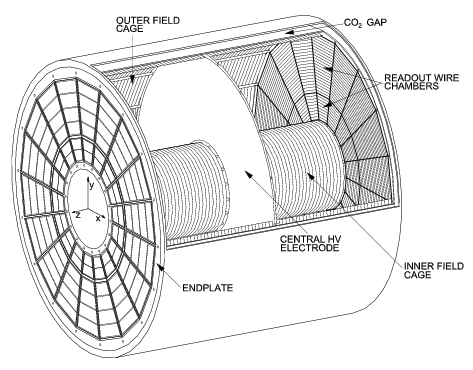
\includegraphics[scale=0.5]{figures/tpc.png}
  \caption{The setup of the TPC.}
  \label{fig:TPC}
\end{figure}
%
The TPC is the main tracking detector of the central barrel. It is optimised to provide momentum measurements with good two-track separation, particle identification via \textit{dE/dx} and vertex determination together with the other detectors of the central barrel. The TPC covers the pseudorapidity range |$\eta$| < 0.9 for tracks with full radial length, i.e. with matches in ITS, TRD and TOF detectors. The 2$\pi$ acceptance in the azimuthal angle is guaranteed by its cylindrical symmetry. The total active volume has an inner radius of 85 cm, an outer radius of 250 cm and a total length along the beam direction of 500 cm. The detector is made of a cylindrical field cage, with a central high-voltage electrode and two opposite axial potential dividers to create a highly uniform electric field. The cavity is filled with 90 m$^3$ of Ne/CO$_2$/N$_2$ (90/10/5).\\
When a charged particle passes through the TPC ionizes the gas creating electron-ion pairs. Thanks to the uniform electric field, the electrons drift towards the end-plates, where they are detected.
The gas mixture is therefore optimised for drift speed, low diffusion, low radiation length and hence low multiple scattering, small space charge effects and stability properties. In particular the N$_2$ improves the quenching of the electron multiplication, keeping the proportionality of the signal to the energy deposit of the charged particles and allowing a higher maximum gas gain. As far as the Ne/CO$_2$ is concerned, the drift speed is strongly dependent on its temperature and therefore a high thermal stability is required ($\Delta$T $\leq$ 0.1 K).\\
In the end-plates the electrons are detected by multi-wire proportional chambers with cathode pad readout, providing the position in the transverse plane. The information about the z position is provided by the measure of the drift time, for which it is necessary to use a trigger information from an external detector, like the V0. The position resolution is different  along the radial direction because of the different track density: for the inner/outer radii is 1100/800 $\mu$m in the transverse plane and 1250/1100 $\mu$m along the beam axis.
%
\begin{figure}
  \centering
  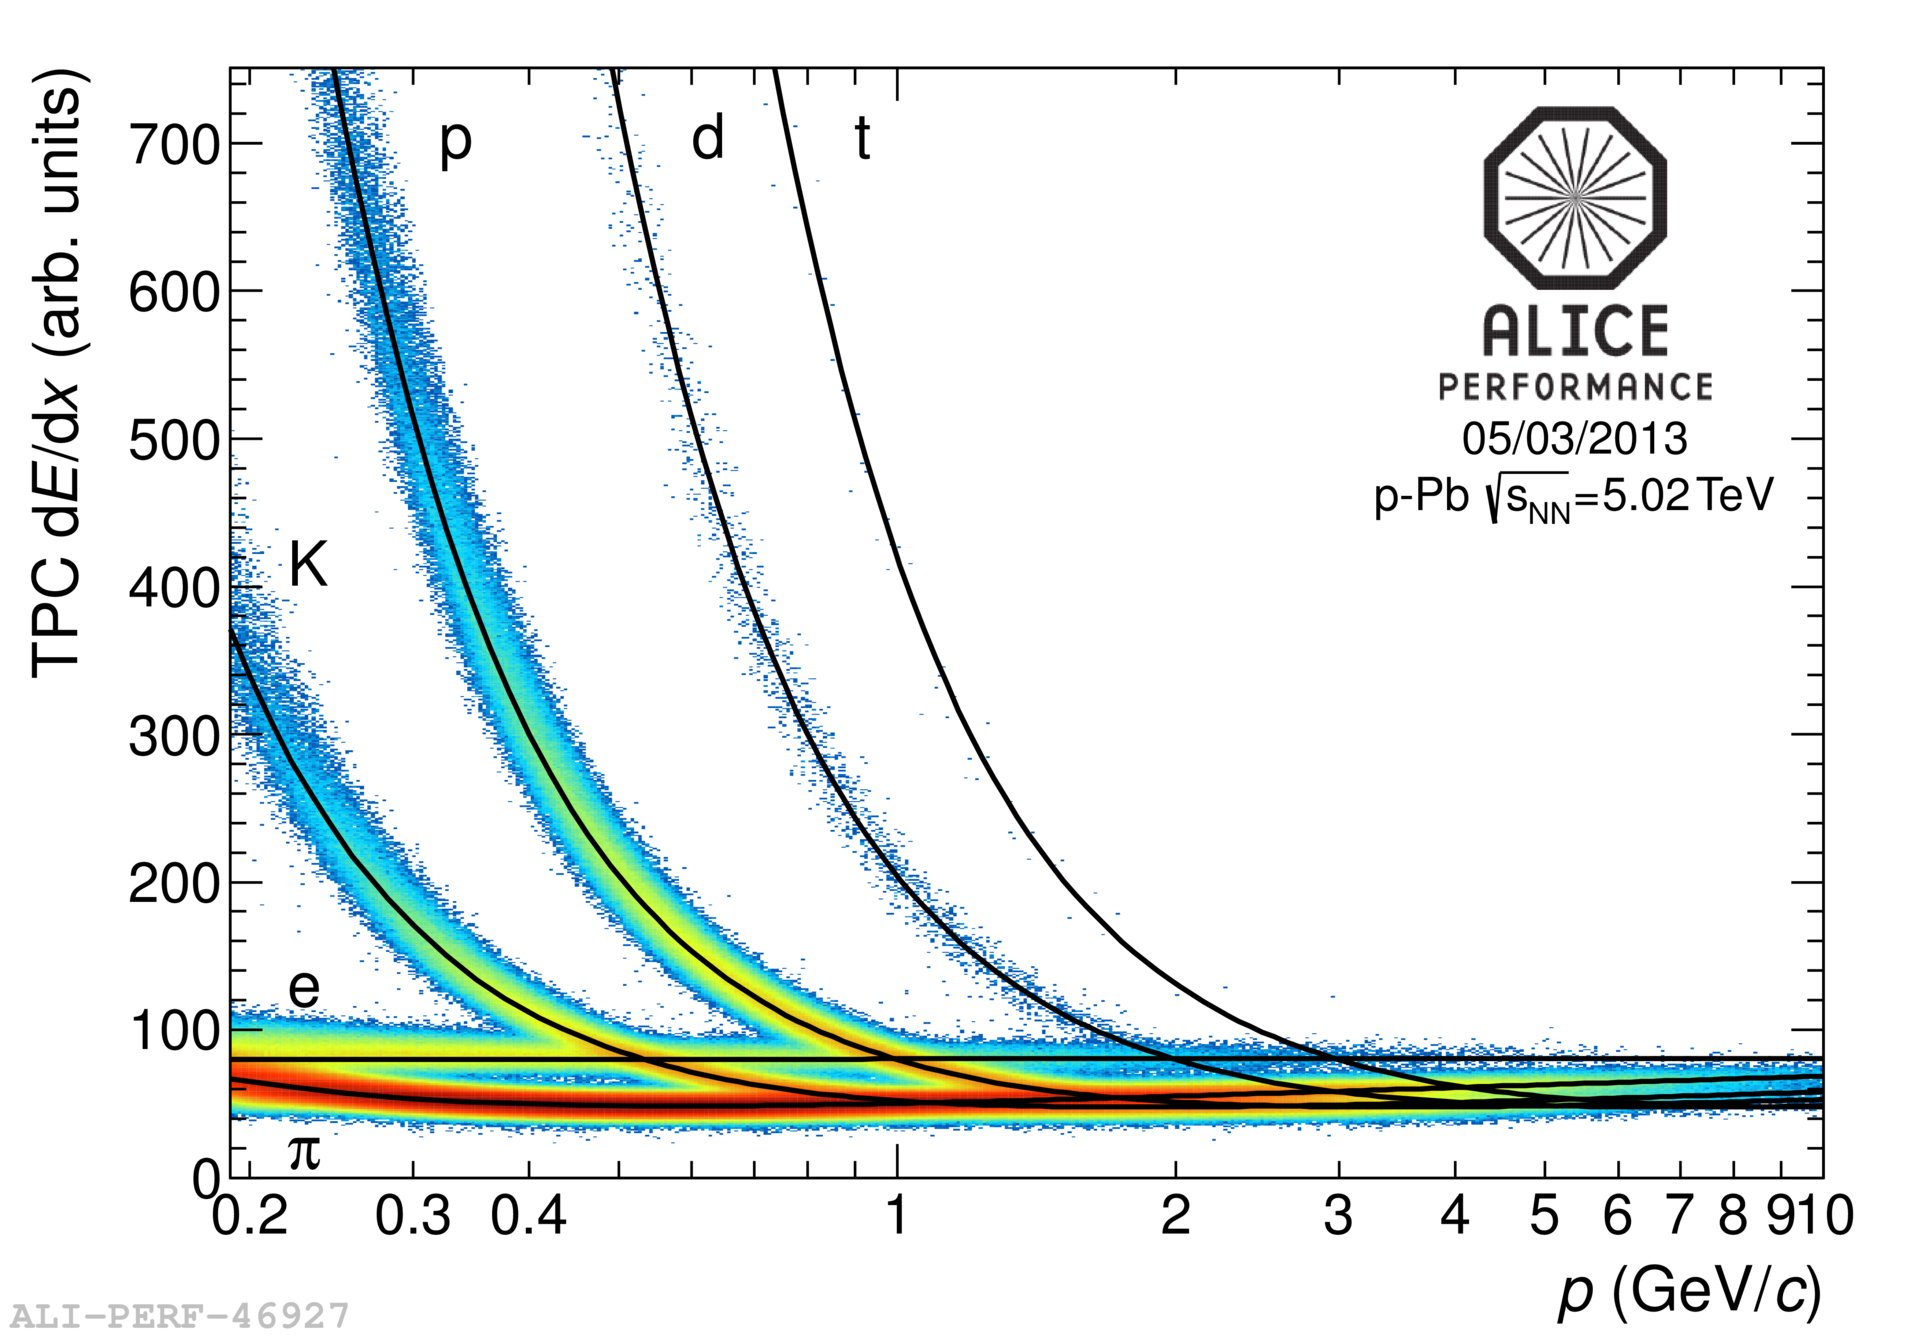
\includegraphics[scale=0.15]{figures/TPC_Perf.png}
  \caption{\textit{dE/dx} of charged particles vs their momentum measured by the TPC in p-Pb collisions. The lines are a parametrization of the detector response based on the Bethe-Bloch formula \cite{alice2014performance}.}
  \label{fig:TPC_Perf}
\end{figure}
%
The total charge collected at the end-plates is proportional to the energy loss of particles in the gas mixture and therefore the PID is possible via \textit{dE/dx}. In particular the \textit{dE/dx} resolution is 5\% for isolated tracks and 6.8\% in case of high occupancy. From \textit{dE/dx} measurements it is possible to identify different particles species in the momentum region where their \textit{dE/dx} are separated. This separation is better at low momentum (p $\lesssim$ 1 GeV/c), where the bands are more distant, but it is possible also at large values of the momentum (p $\gtrsim$ 4 GeV/c) thanks to the relativistic rise of \textit{dE/dx} in the TPC gas.\\
The TPC is a very good detector for tracking and PID, but the large drift time (88 $\mu$s), of the order of 10$^{-3}$, is a great limit for the data acquisition rate.\\
\subsection*{Transition Radiation Detector}
The TRD is used for identifying electrons with momentum above 1 GeV/c, for which the identification in the TPC by measuring the \textit{dE/dx} is no longer efficient. This detector is composed of 540 individual readout detector modules, with an inner radius of 2.9 m and an outer radius of 3.68 m. It works in the pseudorapidity range |$\eta$| < 0.84. The TRD is important, for example, for the separation of the electrons from the J/$\Psi$ decay from the background of Dalitz decays. Moreover combining the information about the impact parameter from the ITS and the identification from the TRD it is possible to study charmed particles with decaying in their semi-leptonic channels. The TRD is composed of radiators in which photons are emitted at charged particle passage and of wire chambers filled wit Xe/CO$_2$. It is suitable for the identification of particles with a Lorentz $\gamma$ larger than 1000 and for this reason it can separate well electrons and pions whose momentum is in the range 1 GeV/c $\leq$ p $\leq$ 100 GeV/c.
\subsection*{Time Of Flight}
The TOF detector consists of a large area array of Multi-gap Resistive Plate Chambers (MRPC) in the central pseudorapidity range (|$\eta$| < 0.9). It is used for the PID in the intermediate momentum range, up to 2.5 GeV/c for pions and kaons, up to 5 GeV/c for protons. It has a cylindrical symmetry like the TPC, with an internal radius of 370 cm, an external one of 399 cm and a total length of 7.45 m. The thickness of the whole detector corresponds to 30\% of a radiation length. When a charged particle passes through the detector ionizes the gas creating an electron avalanche which is collected by the electrodes. The avalanche regime is possible thanks to the high electric fields inside the MWPC.\\
%
\begin{figure}
  \centering
  \includegraphics[scale=0.15]{figures/TOF.png}
  \caption{$\beta$ vs momentum of charged particles measured by the TOF in p-Pb collisions \cite{alice2014performance}.}
  \label{fig:TOF}
\end{figure}
%
The PID is based on the measure of the time of flight of a particle from the interaction point to the TOF detector. Using the track length measured with the ITS and the TPC and using as initial time the time of particle production, provided by the T0 detector, it is possible to measure the $\beta$ of the particle and, considering the momentum measure of the TPC, to identify the particle itself.\\
\subsection*{High Momentum Particle Identification Detector}
\begin{figure}
  \centering
  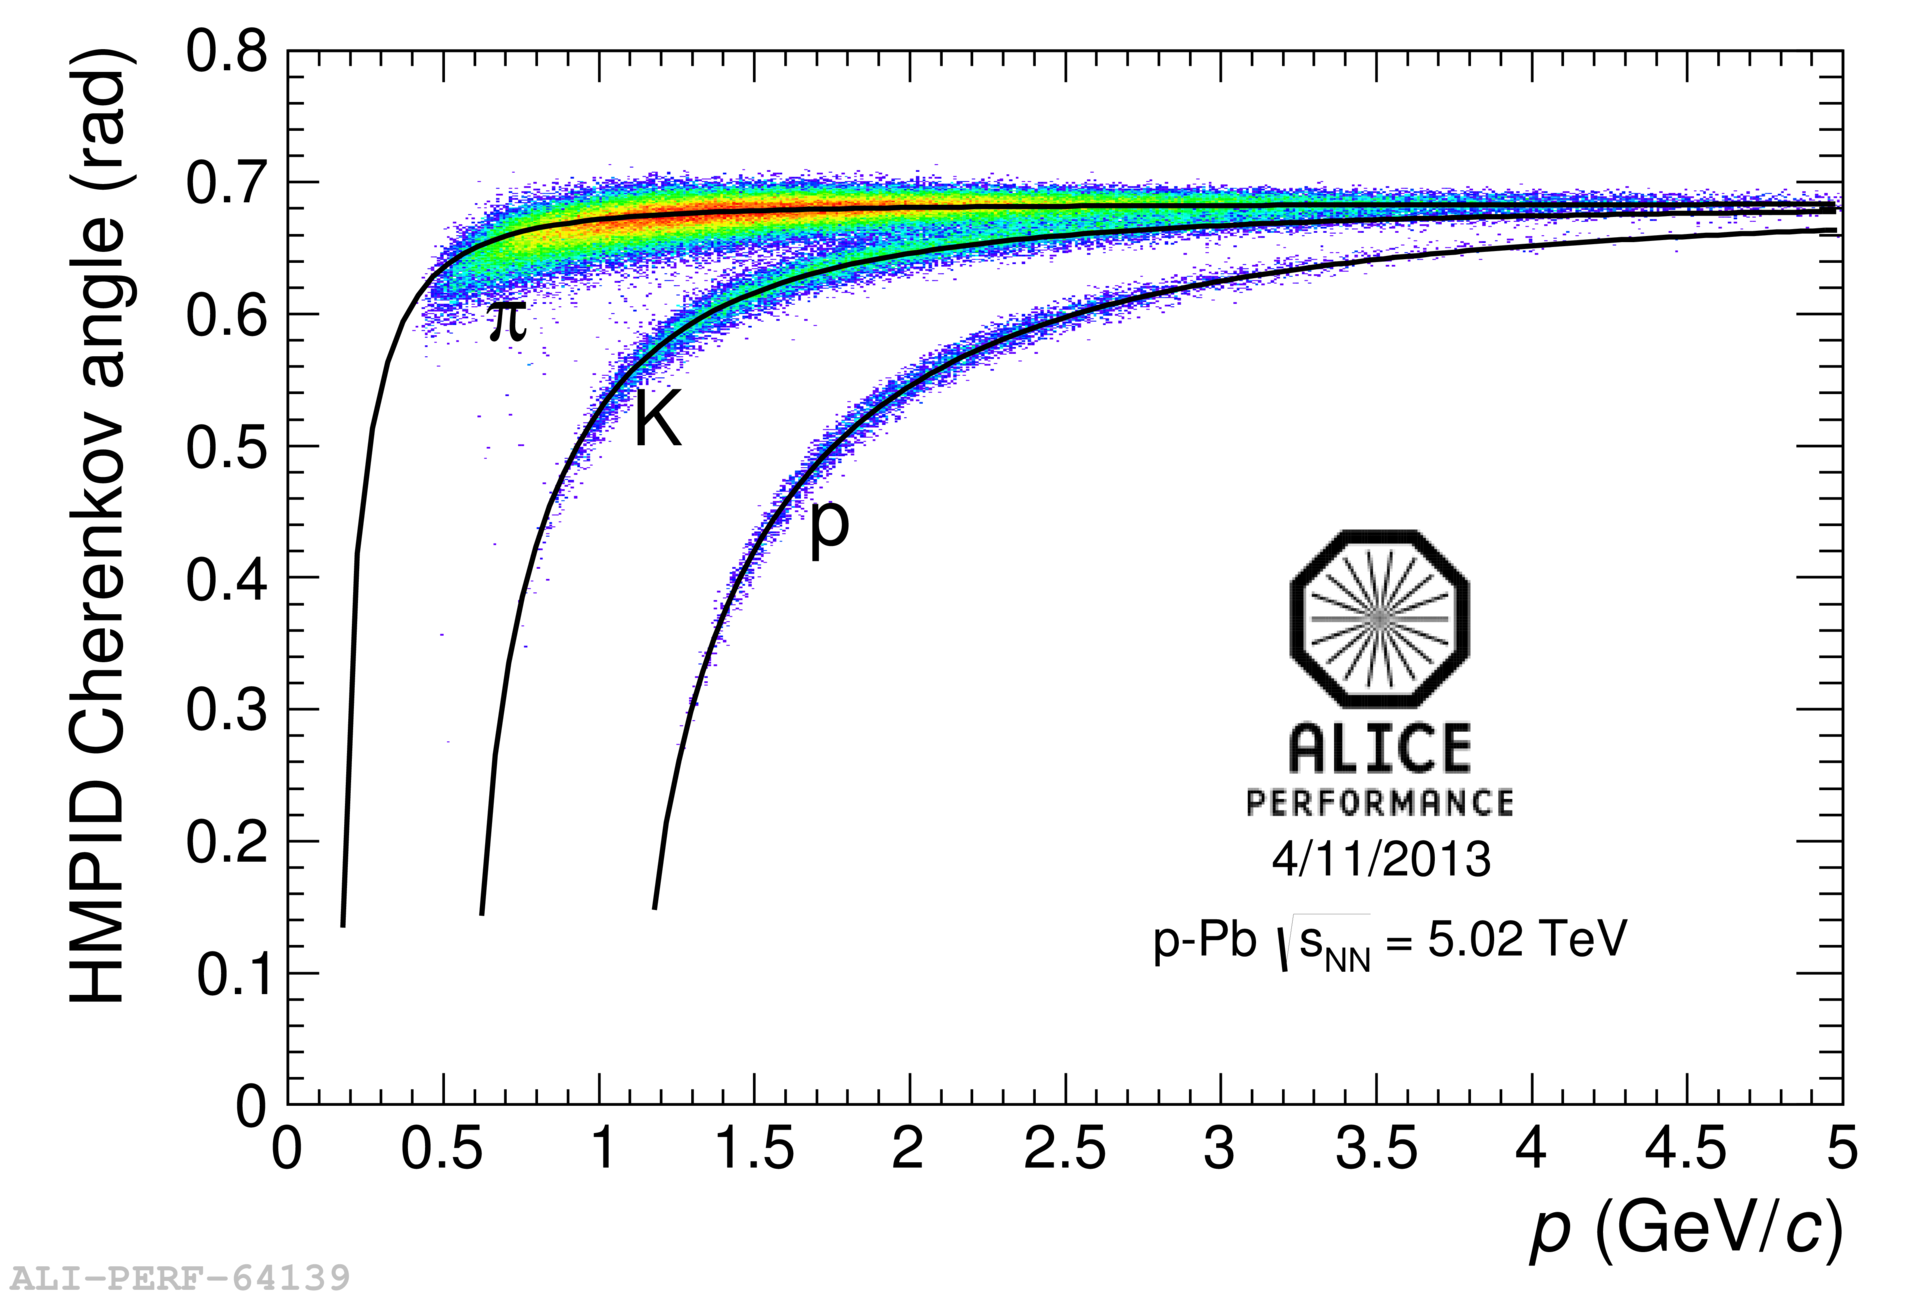
\includegraphics[scale=0.15]{figures/HMPID.png}
  \caption{HMPID Cherenkov angle vs track momentum for p-Pb @ 5.02 TeV data, Continuous lines represent theoretical Cherenkov angle values vs track momentum \cite{alice2014performance}.}
  \label{fig:HMPID}
\end{figure}
%
The HMPID is dedicated to the identification of hadrons at $\pt$ > 1 GeV/c, enhancing the PID capability of ALICE beyond the momentum interval attainable with ITS, TPC and TOF. In particular it has been optimized to extend the range for $\pi$/K and K/p discrimination respectively up to 3 GeV/c and 5 GeV/c. It is characterized by a small acceptance, 5\% of central barrel phase space, covering the pseudorapidity range |$\eta$|<0.6 and the azimuthal angle range 1.2\textdegree < $\varphi$ < 58.8\textdegree. The HMPID is based on proximity-focusing Ring Imaging Cherenkov (RICH) and consists of seven modules of about 1.5 $\times$ 1.5 m$^2$ each, mounted at a distance of about 5 m from the beam line. When a charged particle passes through the radiator, filled with liquid perfluorohexane (C$_6$F$_{14}$), with a speed higher than the speed of light in the medium, Cherenkov photons are emitted. The Cherenkov photons are then detected by a photon counter made of CsI scintillators and a MWPC with pad cathode.
\subsection*{Photon Spectrometer}
The main physics objective of the PHOS is the test of thermal and dynamical properties of the initial phase of the collision through the measurement of low $\pt$ direct photons and of the jet quenching, which can be obtained observing high-$\pt$ $\pi^0$ and $\gamma$-jet correlations. In order to distinguish the direct photons from those generated in $\pi^0$ and $\eta$ decays, good spatial and energetic resolution are needed. The detector consisted of five modules of lead-tungstate crystals (PbWO$_4$) and it is located at 4.6 m from the beam line. It has a low acceptance, covering the pseudorapidity range |$\eta$|<0.12 and the azimuthal angle range 220\textdegree < $\varphi$ < 320\textdegree.
\subsection*{Electromagnetic Calorimeter}
The main goal of the EMCal is to enhance ALICE performances in the the study of the jet production in Pb-Pb collisions. It extends the ALICE capabilities in detecting direct photons, jets and the electrons from heavy flavoured hadron decays. It provides complementary measurements to the PHOS, being positioned approximately in the opposite side, at a radius of about 4.5 m, adjacent to the magnet. It covers the pseudorapidity range |$\eta$|<0.7, with an azimuthal angle range $\Delta\varphi$ = 107\textdegree. The detector is a layered Pb-scintillator sampling calorimeter, alternating 1.44 mm of lead and 1.76 mm of polystyrene.
\subsection*{ALICE Cosmic Ray Detector}
The ACORDE is an array of plastic scintillator counters placed on the upper surface of the L3 magnet and is used for the cosmic ray detection. It covers |$\varphi$| < 60\textdegree $\;$and |$\eta$| < 1.4 range and is positioned at a radius of 8.5 m. It plays a two-fold role in ALICE: the first is to provide a fast trigger signal for the commissioning of the apparatus, calibration and alignment procedures of the tracking detectors; the second is the detection, in combination with the TPC, the TRD and the TOF, of atmospheric muons to study high-energy cosmic rays in the in the energy region around the knee in the cosmic ray spectrum.
\subsection*{Muon Spectrometer}
The Muon Spectrometer allows to reconstruct heavy quarkonia (charmonium and bottomonium states), as well as the $\phi$ meson, through their $\mu^+\mu^-$ decay channel at forward rapidity. The detector covers the pseudorapidity region -4.5 < $\eta$ < -2.5 and consists of different components. In front of the detector itself there is a passive front absorber to screen the detector from hadrons and photons coming from the interaction point. The absorber is made of carbon and concrete, materials characterized by a low atomic number Z to balance screening necessities with the statistical error caused by the multiple scattering of the muons. The absorber is 4.13 m long, corresponding to  $\sim$ 60 X$_0$. After the absorber a high granularity tracking system made of ten detection planes, called \textit{tracking chambers} can be found. The tracking chambers consist of multi-wire proportional chambers with a pad cathode readout, in order to guarantee the high spatial resolution (100 $\mu$m) needed to separate the invariant mass spectra of the dimuons from quarkonia decay. For example, since the masses of the J/$\Psi$ and the $\Psi$' mesons are very close, a resolution of 70 MeV/c$^2$ around the value of 1 GeV/c$^2$ is needed. Similarly, a resolution of 100 MeV/c$^2$ around the value of 100 GeV/c$^2$ is needed to separate the $\Upsilon$ and the $\Upsilon$' mesons. Positive and negative muons are separated by the dipole magnet. In particular, the tracking chambers are arranged in five stations: two before, one inside and two after the dipole magnet. Then, the \textit{inner beam shield} protects the chambers from background originating from particles at small angles. It is made of tungsten, lead and stainless steel to minimize the background arising from primary particles emitted in the collision and from their showers produced in the beam pipe and in the shield itself. Finally, there is the trigger system, designed to select heavy quark resonance decays. The selection is made on the $\pt$ of the two individual muons. It consists of four planes of RPCs, arranged in two stations and positioned behind a passive muon filter, providing the transverse momentum of each muon.
\subsection*{Zero Degree Calorimeter}
The ZDC consists of two pairs of hadronic calorimeters (one for protons and one for neutrons) located at 116 m on each side of the interaction point, along the beam line. The ZDC provides information about the centrality of Pb-Pb collisions measuring the energy of the spectator nucleons. At the LHC indeed it is possible to parametrize the dependence of the energy collected in the ZDC on the number of spectators with the formula:
\begin{equation*}
 E_{ZDC} = \sqrt{s_{NN}} \times N_{spectators}
\end{equation*}
This formula is a good approximation in central events, while for peripheral events the nucleon fragmentation is important and consequently some fragments could not be detected, loosing the proportionality between $E_{ZDC}$ and $N_{spectators}$.\\
The calorimeters consists of tungsten as absorber material and quartz fibres as active material: when a particle passes through the passive material creates a shower which produces Cherenkov radiation, which is detected by the active material. The ZDC is also position sensitive and therefore can provide an estimate of the reaction plane in nuclear collisions.
In addition, two small electromagnetic calorimeters (ZEM) are placed at about 7 m from the interaction point on each side of the beam pipe, opposite to the muon arm.
\subsection*{Photon Multiplicity Detector}
The PMD measures the multiplicity and the spatial ($\eta$ - $\varphi$) distribution of photons in the pseudorapidity region 2.3 $\leq \eta \leq$ 3.7. These measurements give estimations of the transverse electromagnetic energy and of the reaction plane. The PMD consists of a large array of gas (Ar/CO$_2$, 30/70) proportional counters in a honeycomb cellular structure and is located at 3.64m from the interaction point.
\subsection*{Forward Multiplicity Detector}
\begin{figure}
  \centering
  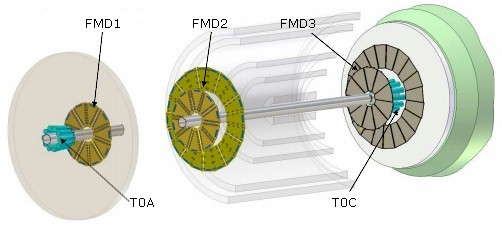
\includegraphics[scale=0.50]{figures/FMD.jpg}
  \caption{FMD and T0 detectors.}
  \label{fig:FMD}
\end{figure}
%
The FMD provides information about the charged particle multiplicity in the pseudorapidity ranges -3.4 $\leq \eta \leq$ -1.7 and 1.7 $\leq \eta \leq$ 5.1. The measurement of charged particle multiplicity is important to study the particle flows and event-by-event multiplicity fluctuations. The FMD is composed of five rings of silicon strip detectors, organized in three components: FMD2 and FMD3 consist of two rings, while FMD1 is made of just one ring. FMD3 is installed on the muon absorber side, FMD1 and FMD2 on the opposite side of the interaction point. FMD2 and FMD3 are placed at about 70 cm from the nominal interaction point, while FMD1 is placed much further from the interaction point, at about 320 cm on the side opposite to the muon arm.
\subsection*{VZERO}
The V0 consists of two arrays of scintillator counters (VOA\footnote{A = ATLAS: it is on the side towards the ATLAS experiment} and VOC\footnote{C = CMS: it is on the side towards the CMS experiment}). The V0A is located 340 cm from the nominal interaction point, on the opposite side to the muon spectrometer, and covers the pseudorapidity range 2.8 < $\eta$ < 5.1. The V0C, instead, is fixed to the front of the hadronic absorber, at 90 cm from the interaction point, and covers the pseudorapidity range -3.7 < $\eta$ < -1.7. Both the detectors cover the full azimuthal angle interval. The V0 has many functions: it provides the \textit{Minimum-Bias} triggers and centrality triggers for Pb-Pb events, it can be used to measure the event multiplicity at forward rapidity, from which the centrality of the event can be determined, it is used for the rejection of background events.
\subsection*{TZERO}
The detector consists of two arrays (T0A and T0C) of Cherenkov counters, placed at -72.5 cm and 375 cm from the interaction point. It covers the pseudorapidity ranges -3.28 < $\eta$ < -2.97 and 4.61 < $\eta$ < 4.92. Its main purpose is the generation of a start time (T0) for the TOF detector, but it can also be used for an independent determination of the vertex position along the beam line, with a precision of 1.5 cm, and to provide the first level (L0) trigger when the position is within the expected value.
\section{Trigger System and Data acquisition}
The trigger system in ALICE is handled by the \textit{Central Trigger Processor} (CTP), which receives trigger inputs from the triggers detectors and sends trigger signals to the readout detectors in case the trigger conditions are fulfilled. It is based on three level of hardware triggers (L0, L1 and L2) and a fourth level (\textit{High Level Trigger}) of software triggers. This multi-level trigger is needed because of the large differences in the readout time of the detectors.\\
Trigger classes (minimum bias, high multiplicity, dimuons) are the combination of the trigger inputs of different trigger detectors, obtained through logical operations with signals. The three trigger levels are characterized by a different response time. The L0 is a fast trigger, with a response time of 1.2 $\mu$s, and uses only detectors characterized by a high readiness, such as SPD\footnote{subdetectors of the ITS, described later}, T0 and V0. If the L0 conditions are matched, the CTP sends the trigger signal to the readout detectors, which start registering the event. The L1 has a response of 6.5 $\mu$s and involves signals from all the detectors: in case after the response time no signal has been received by the CTP, readout detectors stop registering the event. The L2 trigger is the final preliminary check before the data transfer. It looks for specific problems which can spoil, or even make impossible, the reconstruction of the event, like for example the presence of two sequential lead-lead collisions, which would cause a too high occupancy in the TPC. If the L2 requirements are fulfilled, the event can be sent to the \textit{Data Acquisition System}, which manages the data flow from the detectors to the archiving on tape. This process takes place in few steps. First, when the readout electronics of a detector is triggered, it sends data to a farm of 300 individual computers (\textit{Local Data Concentrators}) in the experimental site. Each LDC combines the fragment of data coming from detectors in sub-events. The sub-events are transferred to 40 \textit{Global Data Collectors}, computers that perform the event building. Each GDC is able to process up to 40 events in parallel. At this moment, the data rate coming from the different sub-detectors is about 25 GB/s and the size of a central data can be $\sim$ 70 MB. For this reason the High Level Trigger performs an additional event selection and compression, optimizing the use of recording band available. This data compression allows to reach a data rate of about 1.25 GB/s. Finally, event selected by the HLT are transferred to the CERN computer centre to be recorded on tape.
\section{ALICE Software}
\label{datavol}
The ALICE experiment software is based on ROOT \cite{ROOT}, the data analysis framework developed at CERN. ROOT is an object oriented framework, developed in C++ and characterized by a high flexibility that can be used in many different fields, even if its main applications are in particle physics. A dedicated group at CERN develops and maintains ROOT but many contributions come from the whole particle physicist community, being ROOT an open source project. This framework provides I/O handling functionalities and many advanced statistical tools.\\
The framework adopted by the ALICE offline project is AliRoot \cite{AliRoot}, an object oriented code based on ROOT. The main purpose of AliRoot is to provide a set of software classes and macros to reconstruct and analyse data coming from the ALICE apparatus. For this reason it includes the geometry of the ALICE detectors, their typology and their response to the passage of particles. In addition AliRoot provides the tools for the local reconstruction and analysis of each detector.\\
\begin{figure}
  \centering
  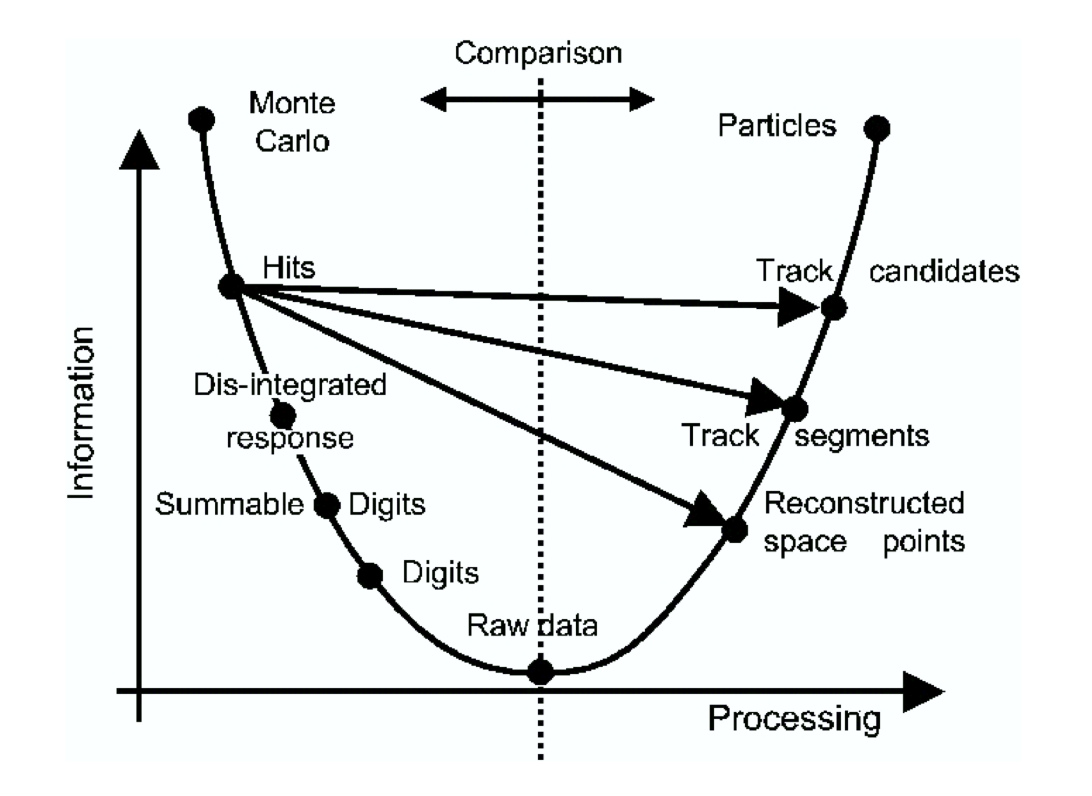
\includegraphics[scale=0.30]{figures/reconstruction.png}
  \caption{Simulation and reconstruction process.}
  \label{fig:Rec}
\end{figure}
%
A scheme of the work flow of the simulation and reconstruction process in AliRoot can be found in Figure \ref{fig:Rec}: the left part shows the simulation steps, followed in the Monte Carlo simulations, while the right part shows the reconstruction steps, common for both real and simulated data.\\
The particles produced in the collision are created using generator codes for heavy-ion interactions such as HIJING \cite{hijing} and PYTHIA \cite{pythia}. The generated particles are  then transported through the detector with transport codes like GEANT3/4 \cite{geant} and FLUKA \cite{fluka}, simulating the interaction with the material and the energy deposit in the active areas of the detectors, which constitutes the particle \textit{hits}. The hit keeps the information about the particle that generated it in form of a \textit{track label}. The next step is the simulation of the response to the hits of the detectors and the readout electronics. The digitization is done in two steps: \textit{summable digits}, produced with low thresholds and used fo the \textit{event merging}, in which signals coming from different events are summed together; \textit{digits}, generated with real trigger thresholds after the noise simulation and are comparable to real raw data.\\
During the reconstruction, digits are extracted from raw data and the adjacent digits are grouped together to form  a \textit{cluster}, which is the signal given by a particle in the detector. \textit{Rec-points} are defined by the reconstructed space position and, where possible, energy deposit. In the next step, the \textit{tracking}, the rec-points generated in the local reconstruction of each sub-detector are associated into \textit{tracks}, which contain the information about the kinematic parameters and the identity of the particles. Finally, the results from the reconstruction step are stored in \textit{Event Summary Data} (ESD, which can be further condensed into an \textit{Analysis Object Data} (AOD), containing the essential information needed for the analysis.
\section{Inner Tracking System}
\label{sec:ITS}
\begin{figure}
  \centering
  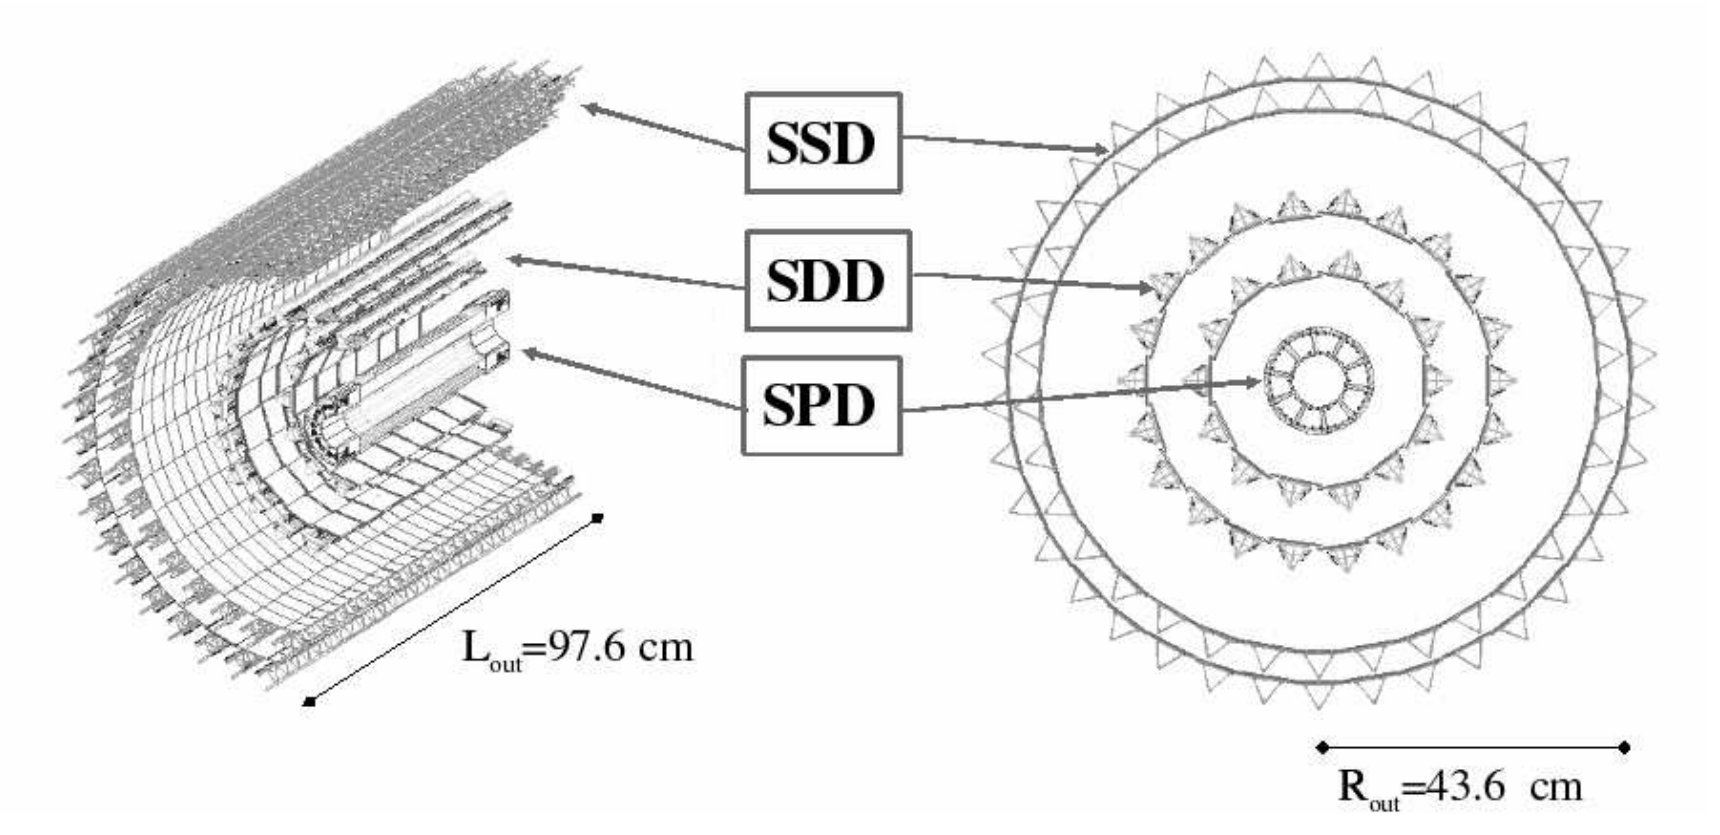
\includegraphics[scale=0.30]{figures/ITS.png}
  \caption{Layout of the ITS.}
  \label{fig:ITS}
\end{figure}
%
The ITS is the closest detector to the interaction point and it consists of six cylindrical layers of silicon detectors of different technologies: the two innermost layers are made of \textit{silicon pixel detectors} (SPD), the two central layers are made of \textit{silicon drift detectors} (SDD) and the two outer layers are made of double-sided \textit{silicon strip detectors} (SSD). The layout of the ITS is schematically shown in Figure \ref{fig:ITS}.\\
The ITS has a full acceptance in the azimuthal angle (2$\pi$) and it covers the pseudorapidity range of |$\eta$| < 0.9 (the same of the TPC) for all the collisions inside the so called \textit{interaction diamond}, the region in which |z| < 5.3 cm. The geometry of the ITS, i.e. the number, the position and the segmentation of the layers, has been optimized for the tracking efficiency and for a high resolution on the impact parameter, which in a decay is defined as the transverse distance of closest approach between a particle trajectory and the primary vertex (an example of impact parameter is shown in Figure \ref{fig:parametro}). The SPD covers a larger pseudorapidity, |$\eta$| < 1.2 for particles generated at z = 0, to provide, together with the FMD, continuous coverage for the measurement of charged particle multiplicity.\\
\begin{figure}
  \centering
  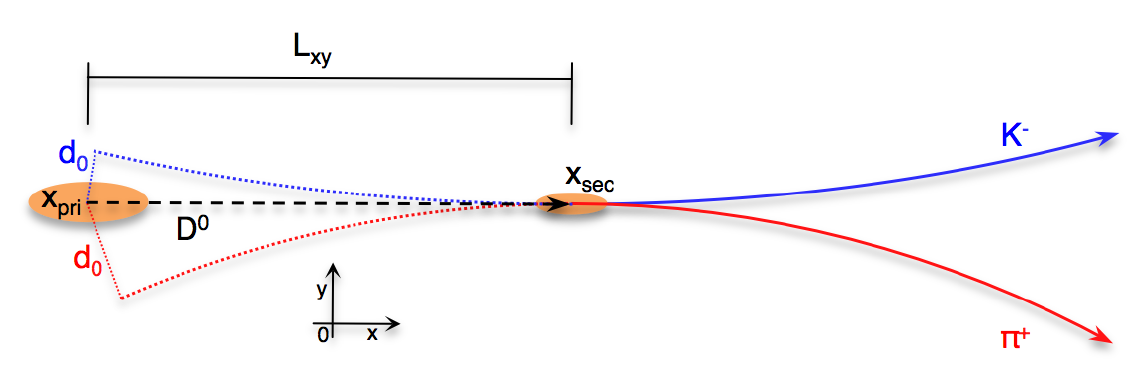
\includegraphics[scale=0.40]{figures/parametro.png}
  \caption{Example of impact parameters in the D$_0$ decay in the transverse plane.}
  \label{fig:parametro}
\end{figure}
%
\begin{table}
\centering
\renewcommand\arraystretch{1.5}
 \begin{tabular}{|c|c|c|c|c|c|}
  \hline
  Layer & Type & r (cm) & $\pm$z (cm) & $\#$ Modules & Material budget ($\%$ of X$_0$)\\
  \hline
  1 & pixel & 3.9 & 14.1 & 80 & 1.14 \\
  2 & pixel & 7.6 & 14.1 & 160 & 1.14 \\
  3 & drift & 15.0 & 22.2 & 84 & 1.13 \\
  4 & drift & 23.9 & 29.7 & 176 & 1.26 \\
  5 & strip & 38.0 & 43.1 & 748 & 0.83 \\
  6 & strip & 43.0 & 48.9 & 950 & 0.86 \\
  \hline
 \end{tabular}
 \caption{ITS geometrical and composition details.}
 \label{tab:ITSgeom}
\end{table}
%
\begin{table}
\centering
\renewcommand\arraystretch{1.5}
 \begin{tabular}{|l|c|c|c|}
  \hline
  Parameter & SPD & SDD & SSD \\
  \hline
  Spacial resolution in $r\varphi$ ($\mu$m) & 12 & 35 & 20 \\
  Spacial resolution in z ($\mu$m) & 100 & 25 & 830 \\
  Two tracks resolution in $r\varphi$ ($\mu$m) & 100 & 200 & 300 \\
  Two tracks resolution in z ($\mu$m) & 850 & 600 & 2400 \\
  Cell size ($\mu$m$^2$) & 50 $\times$ 425 & 202 $\times$ 294 & 95 $\times$ 40000 \\
  Active area per module (mm$^2$) & 12.8 $\times$ 69.6 &  72.5 $\times$ 75.3 &  73 $\times$ 40 \\
  Readout channel per module & 40960 & 2 $\times$ 256 & 2 $\times$ 768 \\
  Total number of modules & 240 & 260 & 1698 \\
  Total number of readout channels (k) & 9835 & 133 & 2608 \\
  Total number of cells (M) & 9.84 & 23 & 2.6 \\
  Max. occupancy (inner layer) (\%) & 2.1 & 2.5 & 4 \\
  Max. occupancy (outer layer) (\%) & 0.6 & 1.0 & 3.3 \\
  \hline
 \end{tabular}
 \caption{Parameters of the various detectors. The maximum occupancy is referred to the most central Pb-Pb collisions. In the ITS a module consists of a sensor element equipped with its front end electronics.}
 \label{tab:ITSparam}
\end{table}
%
The geometrical dimensions and the technologies used in the layers can be found in Table \ref{tab:ITSgeom}, while a list or the ITS characteristics can be found in Table \ref{tab:ITSparam}.\\
The SPD for the two inner layers as well as the SDD for the two middle ones have been chosen because of the high particle density expected in heavy-ion collisions at LHC (about 50 particles for cm$^2$ predicted for the innermost layer) and in order to achieve the needed impact parameter resolution.\\
The four outer layers (SDD and SSD) have an analogue  readout of the charge deposition and therefore can be used for the PID through the measurement of the $dE/dx$ in the non relativistic region of the Bethe-Bloch curve, where $dE/dx \propto 1/\beta^{2}$. For this reason the analogue readout has a large dynamic range to provide the $dE/dx$ for low-momentum particle, which are heavily ionising. This characteristic makes the ITS stand-alone a low-$\pt$ particle spectrometer.\\
Since for low momentum particles the multiple scattering can easily spoil the impact parameter resolution, the material budget of the ITS has been kept to a minimum. For the SDD and the SSD, which are also used to measure the energy deposit, have a minimum thickness of 300 $\mu$m to provide an acceptable signal-to-noise ratio. Also the additional material, such as electronics, cabling, supporting structures has been kept at comparable levels, so that a particle that passes through the whole ITS perpendicularly would traverse $\sim$ 8\% of a radiation length.\\
The ITS design has been optimized to keep good tracking efficiency in a high multiplicity environment, as expected in Pb-Pb collisions at the nominal energy of the LHC. For this reason the granularity of the detector has to be sufficiently high to guarantee a low occupancy, at the level of few  per cent. To achieve this requirement, several millions of active cells in each layer of the ITS are needed, as it can be seen in Table \ref{tab:ITSparam}. The highest granularity is reached in the two innermost layers with SPD,  but a good granularity is reached in the middle layers with SDD too. In the last two layers with SSD the track density is lower and therefore the granularity is lower too.\\
The spatial resolution needed is set by the $c\tau$ of the D mesons, which is of the order of 100 $\mu$m. The ITS has therefore been built with an impact parameter resolution better than 100 $\mu$m in r$\varphi$ plane and a of few tens of mm in z. Moreover, for momenta larger than 3 GeV/c the spatial precision of the ITS is an essential element of the momentum resolution.
\begin{figure}
  \centering
  \subfloat[][]
  {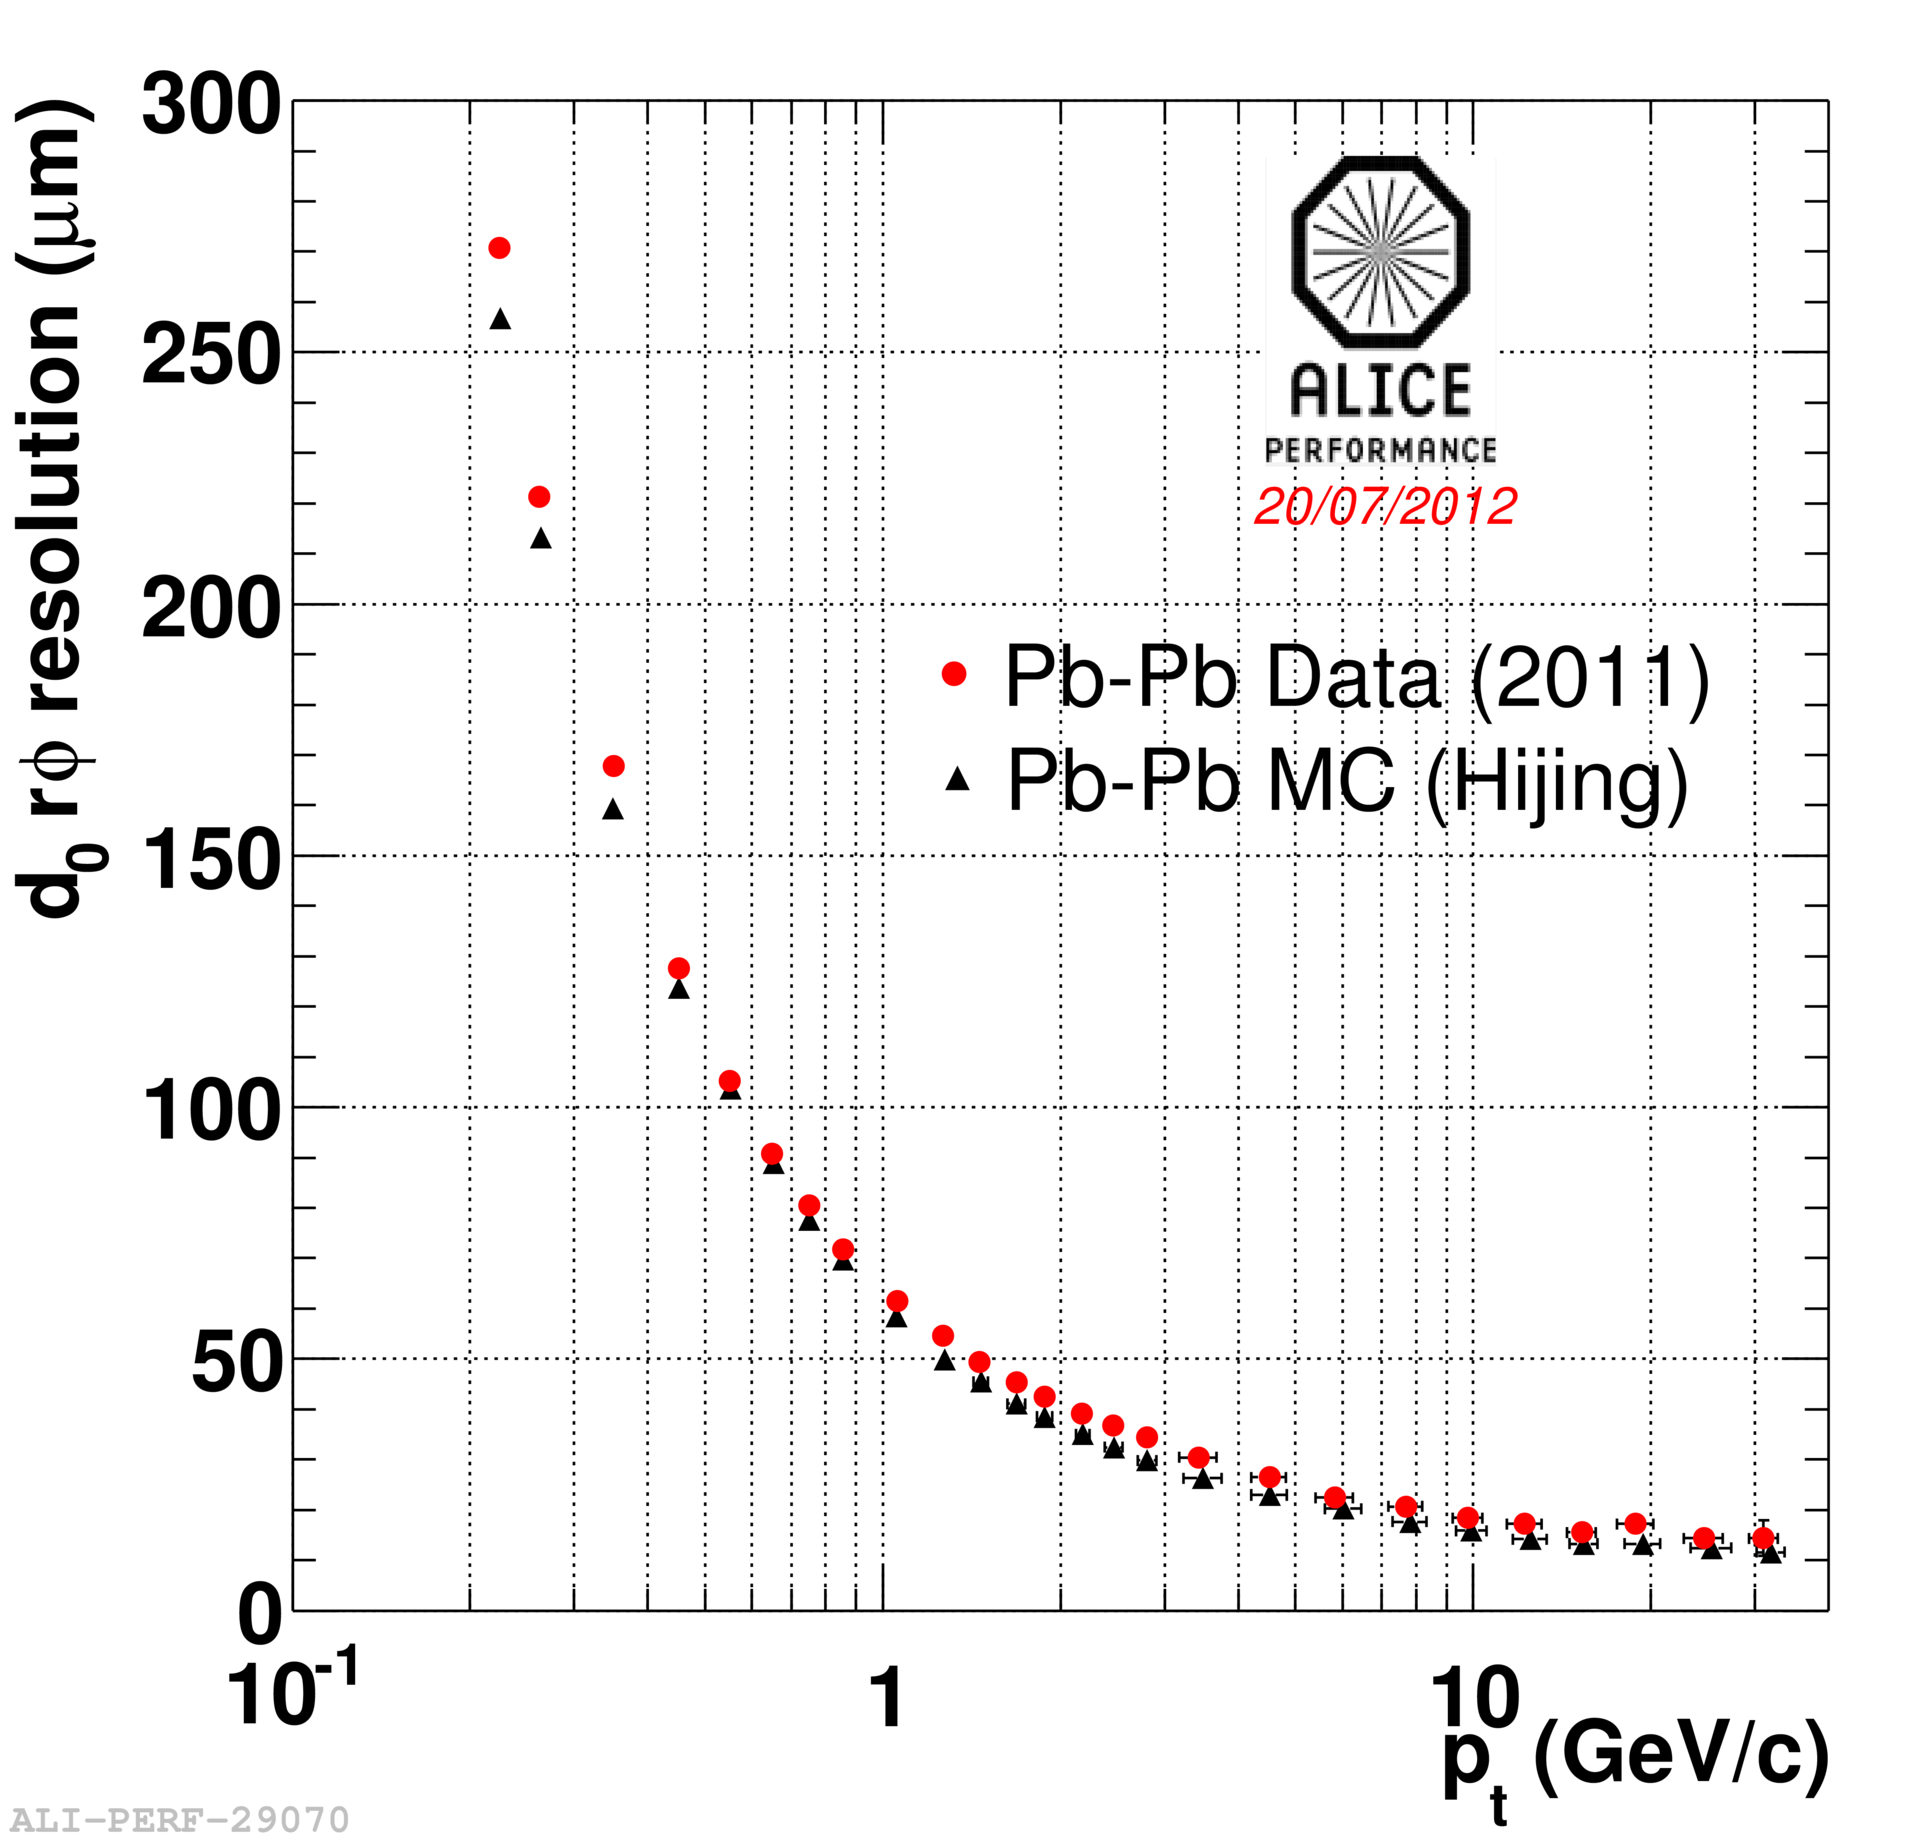
\includegraphics[scale=0.10]{figures/d0rphi.png}\label{fig:d0rphi}}\quad
  \subfloat[][]
  {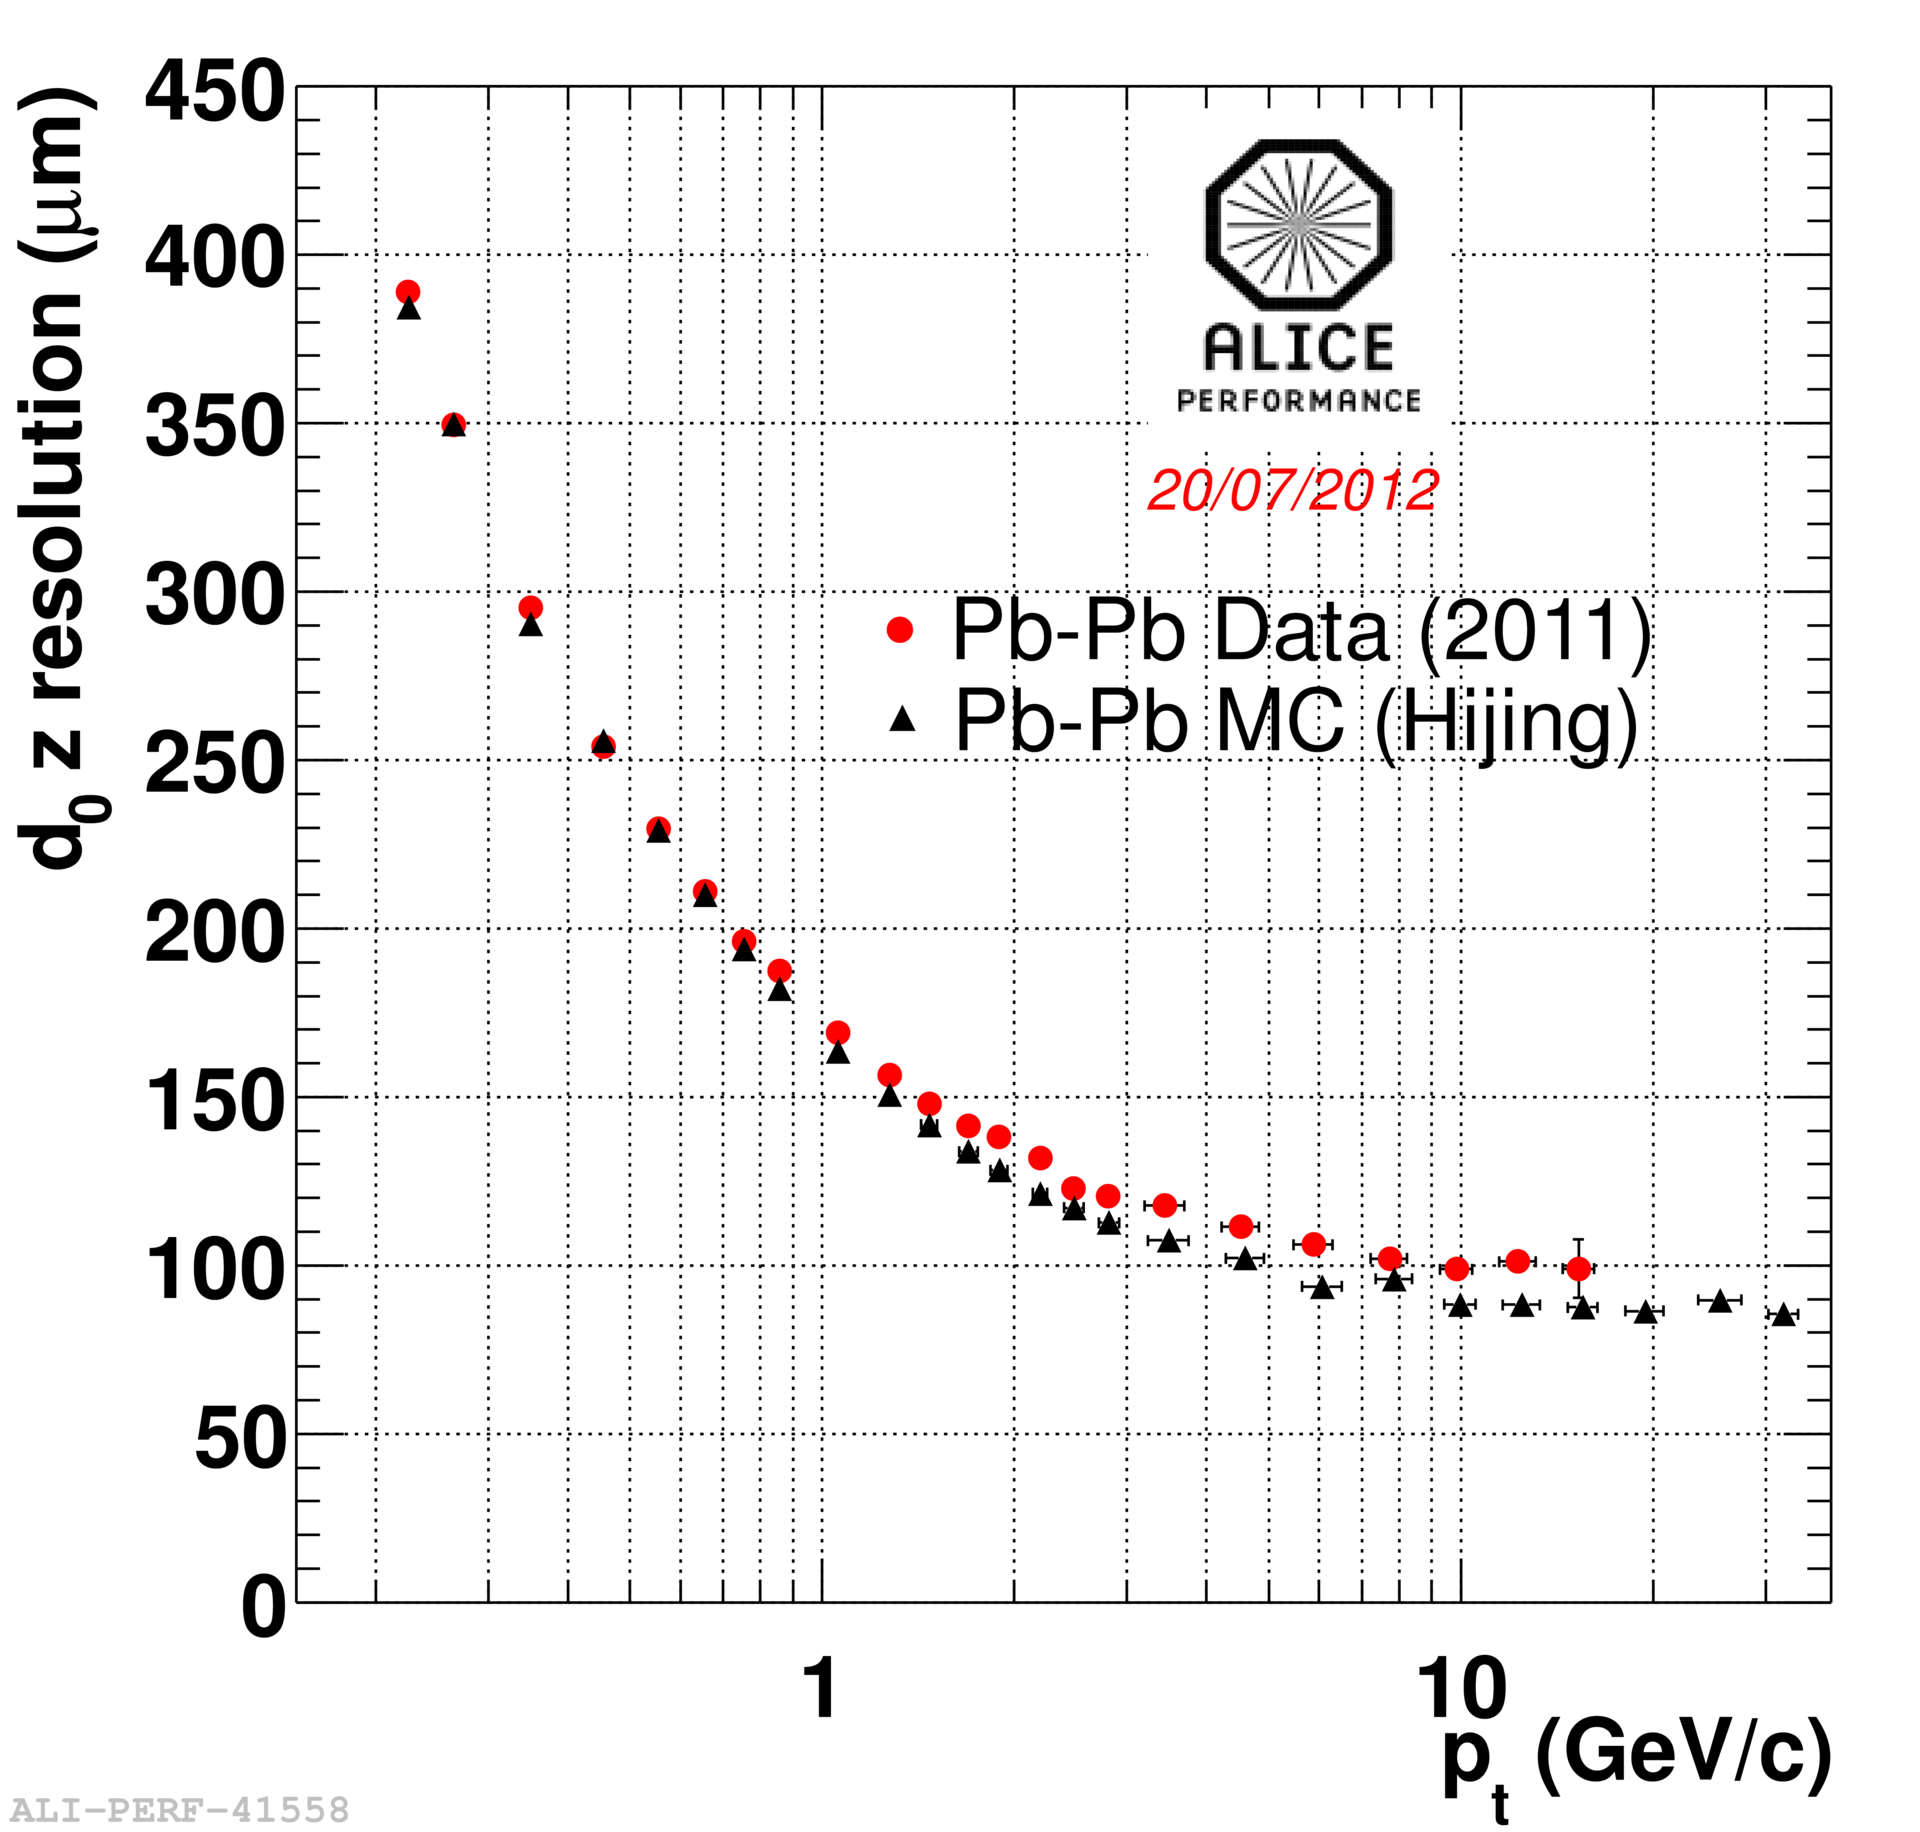
\includegraphics[scale=0.10]{figures/d0z.png}\label{fig:d0z}}
  \caption{Track impact parameter resolution in the transverse plane (a) and in the beam direction (b) in Pb-Pb 2011.}
\end{figure}
The impact parameter resolution as a function of the transverse momentum in r$\varphi$ and z can be seen in Figure \ref{fig:d0rphi} and \ref{fig:d0z}. In both the directions the resolution increases when the transverse momentum of the particle increases, reaching a value better than 20 $\mu$m and 100 $\mu$m in r$\varphi$ and z respectively for $\pt$ values larger than 10 GeV/c.\\
In the next sections the different detectors of the ITS will be described.
\section{Silicon Pixel Detector}
The role of the two innermost layers of SPD is crucial for the determination of the position of the primary vertex as well as for the measurement of the impact parameters of secondary particles originating from the weak decays of particles. The use of a truly two-dimensional detectors brings some advantages. First, the two-dimensional segmentation of the pixel detectors avoids the ghost hits that typically affect the double-sided strip detectors giving an ambiguous information about the hit points. Then, the small dimension of the single pixel (50 $\times$ 425 $\mu$m$^2$) gives a high spatial resolution, combined with a low diode capacitance, which implies an excellent signal-to-noise ratio.\\
The SPD is characterized by a binary digital readout: in each cell, a threshold is applied to the pre-amplified and shaped signal and the digital output level changes when the signal is above threshold. The threshold is about 100 electrons per cell.\\
It is divided in modules, which consist of a two-dimensional matrix of silicon pixel detectors, also called sensor ladder, bounded to the related front-end electronics. Each matrix is made of 256 (r$\varphi$) $\times$ 160 (z) pixels, with a total area of 12.8 mm (r$\varphi$) $\times$ 69.6 mm (z). Two modules aligned in z direction form a \textit{half-stave}, whose length is 141.6 mm. Two half-staves are attached head-to-head laong the z direction to a carbon fibre support sector to form a stave. Each sector supports six staves and provides the cooling for the detectors.\\

\section{Silicon Drift Detector}
\begin{figure}
  \centering
  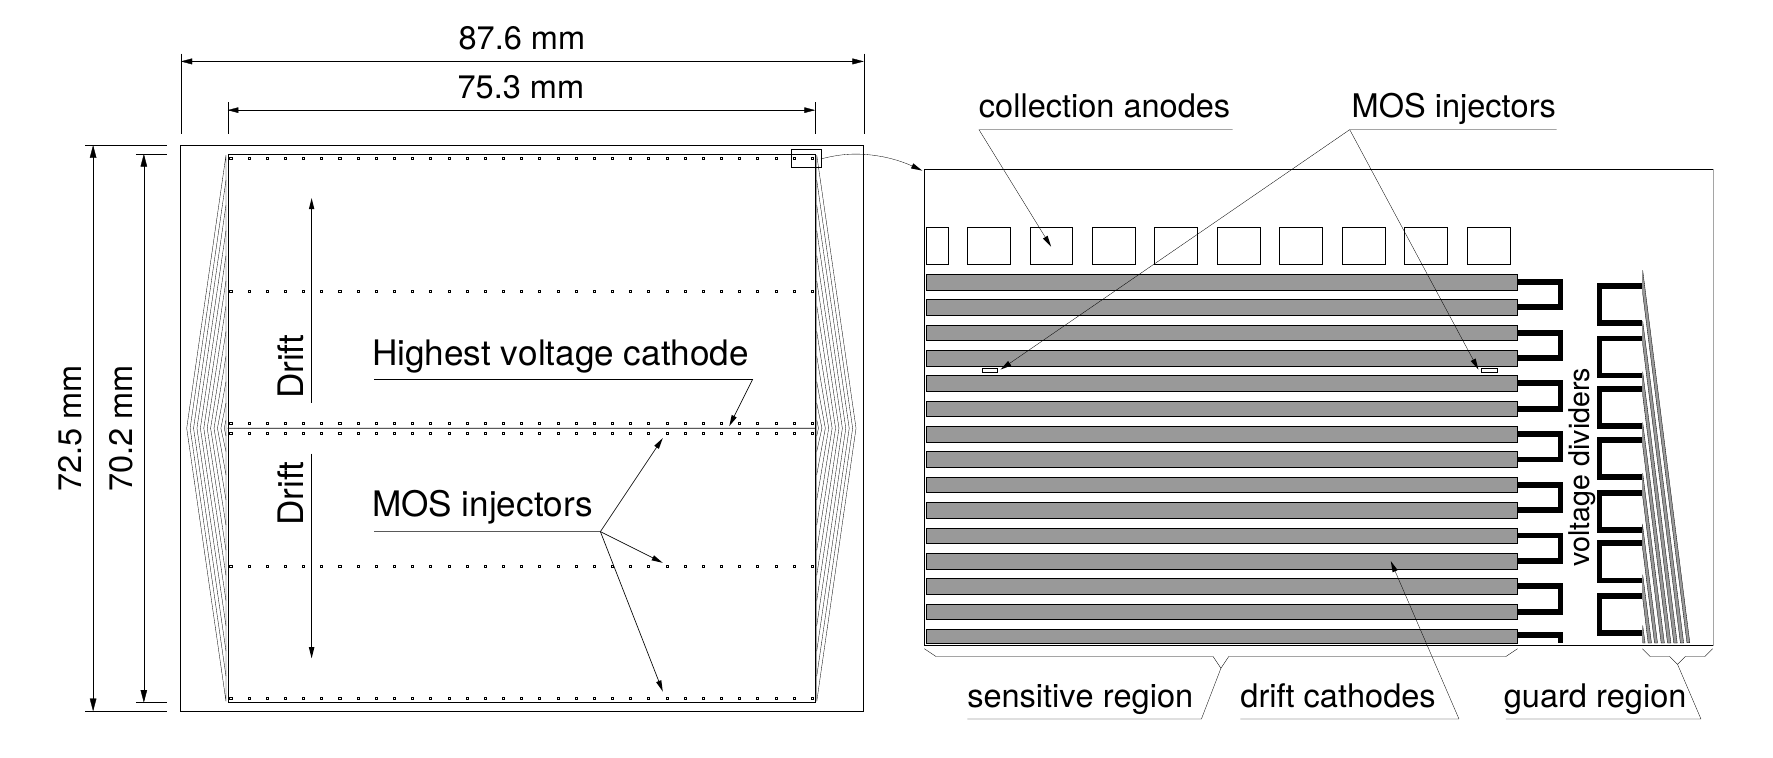
\includegraphics[scale=0.30]{figures/SDD.png}
  \caption{Layout of the ALICE SDD.}
  \label{fig:SDD}
\end{figure}
%
\begin{figure}
  \centering
  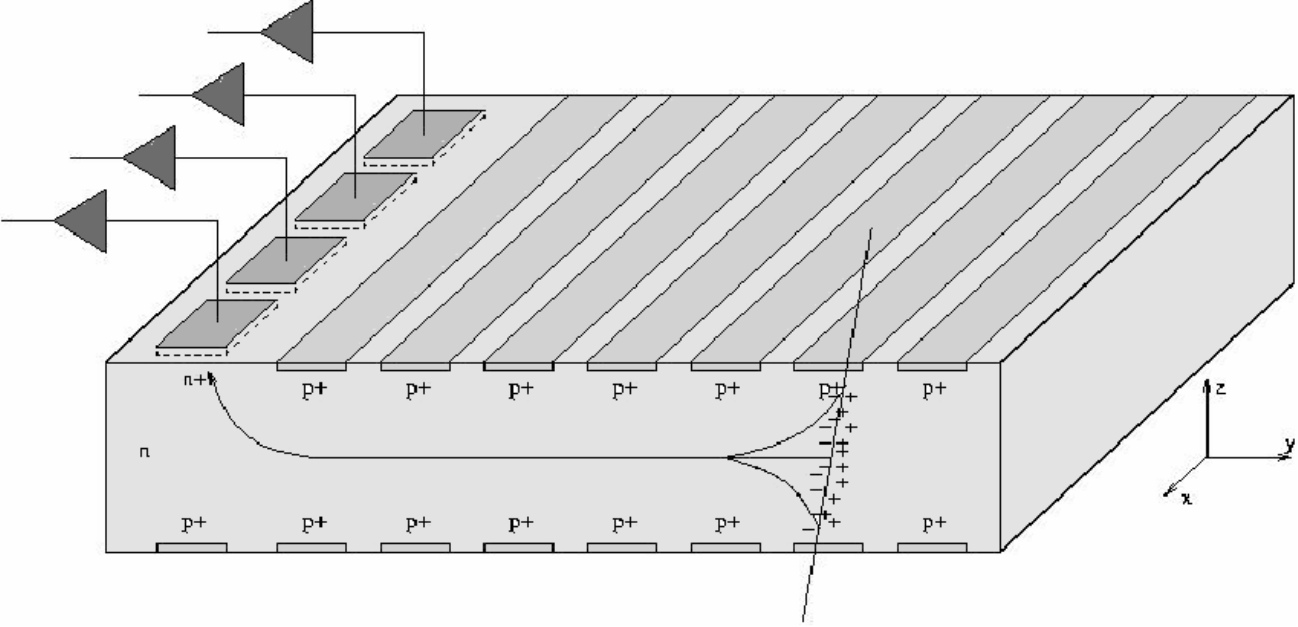
\includegraphics[scale=0.25]{figures/sddw.png}
  \caption{Representation of the working principle of the SDD.}
  \label{fig:sddw}
\end{figure}
%
The SDD constitutes the two intermediate layers of the ITS and is located in a region where the charged particle density is lower than for the SPD. The layout of a SDD can bee seen in Figure \ref{fig:SDD}. The single drift detector gives a two-dimensional information about the position of the particle. The z-coordinate of the point can be determined by the centroid of the charge collected by the anodes. The position along the r$\varphi$ direction, instead, is obtained measuring the time necessary to electrons, produced by the ionizing particle crossing the detector, to drift to the collecting anodes under the effect of an electric field. The drift time is measured with respect to the trigger time. A representation of the working principle of the SDD can be found in Figure \ref{fig:sddw}.\\
The SDDs are produced from 300 $\mu$m thick silicon wafers, characterized by a high resistivity (3 k$\Omega$cm) and a good doping homogeneity (5\%). They have a sensitive area of 70.17 (r$\varphi$) $\times$ 75.26 (z) mm$^2$ and a total area of 72.50 (r$\varphi$) $\times$ 87.59 (z) mm$^2$. The sensitive area is split into two drift regions by a central cathode strip, with a high voltage bias of -1.8 kV. On each surface of the drift region, 291 p$^+$ cathode strips, with 120 $\mu$m pitch, fully deplete the detector volume and generate a drift field parallel to the surface. The drift field is obtained with a voltage divider located on the detector sides, which scales down the HV applied from the central cathode towards the anodes. Each drift region contains 256 collection anodes with 29a $\mu$m pitch and 33 MOS charge injectors to monitor the drift velocity and, therefore, calibrate the sensor. The drift velocity is dependent on the temperature (v$_{drift} \propto$ T$^{-2.4}$) and for this reason te temperature fluctuations must be limited ($\Delta$T $\leq$ 0.1 K). For a HV of -1.8 kV applied to the central cathode, the drift velocity is 6.5 $\mu$m/ns. Since the front-end electronics samples the signal fo each anod with a rate of 40 MHz, the size of a cell is 294 $\times$ 202 $\mu$m$^2$, corresponding to about 9000 cells for sensor, which are readout by 512 electronics channels. Therefore SDD are characterized by a good 2D resolution with a low number of readout channels.\\
Moreover, since the collective charge is proportional to the energy loss of the particle within the sensor, SDDs can also be used for particle identification via \textit{dE/dx}, thanks to the presence of the analogue readout electronics.\\
The signal readout of the SDD is based on three stages. The first, the PASCAL chip, consists of a preamplifier, an analogue storage and an analogue-to-digital converter (DAC) and works at a frequency of 20 MHz. The second stage is AMBRA, which is a digital four-event buffer which performs the baseline equalization on anode-by-anode basis and the 10-bit to 8-bit non-linear data compression. The final stage is CARLOS, which performs the zero-suppression and the data compression. It is very important to underline that the passage of information fron AMBRA to CARLOS take 1.23 ms, but reduce the SDD event size by more than an order of magnitude.\\
Finally, a SDD module consists of one silicon drift detector and two front-end chips. The modules are mounted on linear structures called ladders: there are 14 ladders with six modules each on the third layer and 22 ledders with eight modules each on the fourth layer. The ladders are assembled on a \textit{Carbon Fibre Reinforced Plastic} (CFRP) structure. 
\section{Silicon Strip Detector}
The two outer layers of the ITS are made of double-sided silicon strip detectors. In the ALICE tracking system, the SSD plays an extremely important role in the track propagation from the TPC to the ITS. In addition to the two-dimensional information on the particle position, it provides also information on the collected charged, thanks to the analogue readout electronics. Therefore in the SSD the \textit{dE/dx} information can be used for the particle identification in the low momentum region.\\
The sensors are 300 $\mu$m thick and they have 768 strips on each side, with a pitch of 95 $\mu$m and a length of 40 mm. Sensor are mounted with the strips nearsly parallel to the magnetic field in order to optimize the resolution in the bending direction. Moreover, the sensor p-side (n-side) of layer 5 (layer 6) faces the interaction region, resulting in four almost equally spaced strip orientations in the two layers, which significantly reduces the number of ambiguities seen by the tracking software.\\
A SSD module consists of one sensor connected with two front-end electronic ships. The modules are assembled on ladders of the same design as those supporting the SDD. There are 748 ladders on the fifth layer and 960 on the sixth, for a total number of modules of 1698. The ladders are assembled on a \textit{Carbon Fibre Composite} support structure.\\
The electronic signals from the modules are AC-coupled and buffered in custom made electronics, the \textit{EndCap Modules} (ECM), located at each end of each ladder. The analogue-to-digital conversion of the signals is performed in the \textit{Front-End ReadOut Modules} (FEROM), located outside the ALICE magnet.